\section{The question}\label{sec:question}

Nearly every AI product shipped in 2026 runs on intelligence it does not own. A support bot, a contract reviewer and a coding agent usually all reduce to an HTTP call to one of three companies. The weights sit somewhere else, and so do the prices, the deprecation schedule and the terms of service.

A counter-story has become popular. Open-weight models trail the frontier by months, not years. Fine-tuning a model now costs less than a team lunch. Small specialized models beat giants on narrow tasks. On this story, organizations will stop renting intelligence and start owning it.

This essay tests that story. Its central question:

\begin{quote}
\textbf{Will organizations increasingly own and adapt their AI capabilities rather than exclusively rent them?}
\end{quote}

My answer, defended in what follows, is \emph{yes, but not in the way the story imagines}. Ownership is growing, but it is not a migration from rented frontier models to self-hosted ones. It is a shift in which layer of the stack an organization controls. The layer worth owning is usually not the hardware or even the weights. It is the data, the evaluations and the pipeline that can re-adapt the next base model.

That is the sense of the title. The paradigm taking shape is not owned intelligence replacing rented intelligence, but the two running in parallel. A rented frontier handles open-ended reasoning. An owned adaptation layer beneath it handles the work an organization does most often, or cannot send elsewhere.

\subsection{What is measured here, and what is argued}

The essay combines four kinds of evidence. To keep them apart, important claims carry one of these labels:

\begin{itemize}
\tightlist
\item
  \lbl{Observed} a published measurement or a result from my own experiments, with its source.
\item
  \lbl{Calculated} my arithmetic or model output on sourced inputs, with assumptions stated.
\item
  \lbl{Hypothesis} a reasoned claim that the evidence supports but does not settle.
\item
  \lbl{Speculation} my judgment about the future, offered as such.
\end{itemize}

Prices, market shares and product facts are as of 8 November 2026 and will age quickly. Sourced numbers link to the page they came from. Code, data hashes and random seeds for the original results are listed in Appendix B.

\subsection{What is new here}

Four pieces are, as far as I can tell, original. The \textbf{ownership ladder} separates the rights an organization can hold, so ``ownership is rising'' becomes measurable. A \textbf{dynamic, labor-inclusive break-even model} shows how falling API prices move the point at which owning pays. A \textbf{harm-channel model} of training-data defects separates defects that waste compute from those that damage models or corrupt evaluation. And three \textbf{reproducible experiments} measure detection, framework behavior and harm under controlled defect injection.

\section{The current economics of intelligence}

In late 2026, organizations buy AI in three ways. They call a proprietary API, call an open-weight model hosted per token by a third party, or serve a model on GPUs they rent or own. The first channel takes almost all the money. The second carries a large but volatile share of the work. The third is rarer than the discourse suggests.

\subsection{What intelligence costs per task}

List prices mean little until they are converted into a unit of work. Take a typical narrow task, such as extracting fields from a document or triaging a ticket: about 1,500 input tokens and 200 output tokens. \lbl{Calculated} from list prices on 8 November 2026:

{\small
\begin{longtable}[]{@{}
  >{\raggedright\arraybackslash}p{(\columnwidth - 6\tabcolsep) * \real{0.3776}}
  >{\raggedright\arraybackslash}p{(\columnwidth - 6\tabcolsep) * \real{0.2041}}
  >{\raggedright\arraybackslash}p{(\columnwidth - 6\tabcolsep) * \real{0.2245}}
  >{\raggedright\arraybackslash}p{(\columnwidth - 6\tabcolsep) * \real{0.1939}}@{}}
\caption{Cost of one narrow task (1,500 input and 200 output tokens) at list prices on 8 November 2026. \label{tab:prices}}\tabularnewline
\toprule\noalign{}
\begin{minipage}[b]{\linewidth}\raggedright
Model
\end{minipage} & \begin{minipage}[b]{\linewidth}\raggedright
Input, \$ per 1M tokens
\end{minipage} & \begin{minipage}[b]{\linewidth}\raggedright
Output, \$ per 1M tokens
\end{minipage} & \begin{minipage}[b]{\linewidth}\raggedright
Cost per 1,000 tasks
\end{minipage} \\
\midrule\noalign{}
\endfirsthead
\toprule\noalign{}
\begin{minipage}[b]{\linewidth}\raggedright
Model
\end{minipage} & \begin{minipage}[b]{\linewidth}\raggedright
Input, \$ per 1M tokens
\end{minipage} & \begin{minipage}[b]{\linewidth}\raggedright
Output, \$ per 1M tokens
\end{minipage} & \begin{minipage}[b]{\linewidth}\raggedright
Cost per 1,000 tasks
\end{minipage} \\
\midrule\noalign{}
\endhead
\bottomrule\noalign{}
\endlastfoot
OpenAI gpt-6-astra & 10.00 & 50.00 & \$25.00 \\
Claude Opus 5.5 & 4.00 & 20.00 & \$10.00 \\
Kimi K3 (open, hosted by DeepInfra) & 2.85 & 14.25 & \$7.13 \\
Gemini 3.1 Pro Preview & 2.00 & 12.00 & \$5.40 \\
Claude Sonnet 5.5 & 2.00 & 10.00 & \$5.00 \\
Gemini 3.5 Flash & 1.50 & 9.00 & \$4.05 \\
Gemini 3.1 Flash-Lite & 0.25 & 1.50 & \$0.68 \\
DeepSeek V4.1 Flash (open, DeepInfra) & 0.20 & 0.60 & \$0.42 \\
Qwen3-30B-A3B (open, DeepInfra) & 0.12 & 0.50 & \$0.28 \\
Claude Haiku 5.5 / OpenAI gpt-6-luna & 0.10 & 0.50 & \$0.25 \\
Llama 3.3 70B (open, DeepInfra) & 0.10 & 0.32 & \$0.21 \\
Llama 3.1 8B (open, DeepInfra) & 0.02 & 0.04 & \$0.04 \\
\end{longtable}
}

Sources: \citet{anthropic2026pricing}, \citet{openai2026pricing}, \citet{google2026pricing}, \citet{deepinfra2026pricing}. All three proprietary vendors list batch discounts of about 50\%; for OpenAI I inferred the figure from its price list rather than a stated rule. Vendors tokenize the same text differently, so per-token comparisons across vendors carry an error of tens of percent. Anthropic's price list notes, for example, that Claude 4.7 and later produce about 30\% more tokens for the same text.

The spread is six hundredfold, from 4 cents to \$25 per thousand tasks. Even at the top, a thousand tasks cost less than an hour of an engineer's time.

\subsection{Who sells it, and what the market rewards}

\lbl{Observed} Menlo Ventures' December 2025 survey of 495 US enterprise buyers put Anthropic, OpenAI and Google at 88\% of enterprise LLM API usage between them. It found the open-source share had fallen from 19\% to 11\% over the year and that 76\% of AI use cases were bought rather than built. It also described fine-tuning as still niche \citep{menlo2025}.

Menlo's next survey, fielded in September 2026 with nearly 400 buyers, shows a rebound and a split. Open-source models went back from 11\% to 19\% of enterprise \emph{tokens}, their 2024 level, but fell from 6\% to 4\% of enterprise \emph{spend}. The average open-source token fell 3.3-fold to \$0.13 per million, against a blended closed price of \$0.70 \citep{menlo2026}. On OpenRouter, a developer platform, open-weight models reached about a third of weekly tokens by late 2025 and averaged roughly a quarter over the year \citep{aubakirova2026openrouter}.

Open models are winning the cheap, high-volume work. Closed models are winning where capability is priced, and Menlo concludes that capability, not price, decides purchases. Two cautions apply. These surveys are small, US-only and not probability samples, and Menlo is an investor in Anthropic, one of the three leading labs. And open-model tokens are mostly bought per token from hosts, which is level 0 on the ladder in section 4. They measure use of open models, not ownership of them.

\subsection{Why organizations rent}

The reasons are better than inertia. Capability comes first, and the frontier still sits behind closed APIs, even if open-weight models trail it by only a few months (section 3). The frontier also moves every few months, which makes any model an organization builds a depreciating asset; Menlo names this as a barrier to post-training. Expertise is scarce. And as the table shows, the token bill is often too small to be worth optimizing.

\subsection{Four assumptions that mislead}

\begin{enumerate}
\def\labelenumi{\arabic{enumi}.}
\tightlist
\item
  \textbf{``API inference is the big cost.''} For a narrow task it is usually cents per thousand calls. \lbl{Calculated} At Sonnet 5.5 prices, an organization runs 2 million tasks a month for \$10,000, less than one engineer's monthly cost at US rates. Labor and the cost of errors usually dominate (section 4).
\item
  \textbf{``Open weights are free, so self-hosting is cheaper.''} Hosted open-weight prices sit close to the self-hosting floor. \lbl{Calculated} NVIDIA's TensorRT-LLM benchmark serves about 15,000 output tokens a second for Llama 3.1 8B on one H100, with 1,000 input tokens per request \citep{nvidia2026trtllm}. At the \$3.00 hourly H100 index price, a million input plus a million output tokens cost about \$0.056 at \emph{full} utilization, against \$0.06 for the same traffic at DeepInfra. At the throughput and utilization one organization realistically achieves (section 4.3), the same traffic costs about \$0.31, five times the host's price. An organization is unlikely to undercut a host that batches many customers on the same GPUs.
\item
  \textbf{``Open source is losing'' or ``open source is winning.''} Both are true, depending on whether you count tokens or dollars. Each camp quotes the metric that suits it.
\item
  \textbf{``Fine-tuning is dead.''} a16z's 2025 survey of 100 CIOs found fine-tuning ``viewed as less necessary'' as long context improved \citep{wang2025cio}. Yet Menlo's 2026 survey found the share of AI builders who post-train rose from 6\% to 10\%, and 91\% of them use outside partners. \lbl{Hypothesis} Fine-tuning is not dying. It is moving away from closed vendors' APIs and toward open bases and specialist partners.
\end{enumerate}

\section{The changing economics of adaptation}

The compute cost of adapting a model has collapsed to a few dollars. The total cost has not, because the expensive inputs are now people, data and evaluation. Fine-tuning has become accessible to anyone with a GPU budget. It has become \emph{useful} only to those with the other three.

\subsection{Three different activities}

Pretraining builds a base model from trillions of tokens and remains the preserve of a few dozen labs. Fine-tuning adapts an existing base to a task with thousands to millions of examples. Inference runs the result. Most confusion about ``owning AI'' comes from mixing the first activity's costs into arguments about the second.

\subsection{Why adaptation got cheap}

Low-rank adaptation (LoRA) freezes the base weights and learns a small low-rank update to each layer \citep{hu2021lora}. QLoRA added 4-bit quantization of the frozen base, which put a 65B-parameter model's fine-tuning on a single 48 GB GPU \citep{dettmers2023qlora}. The lingering doubt was whether LoRA's savings cost quality. Thinking Machines' 2025 study found LoRA matches full fine-tuning for small-to-medium supervised and reinforcement-learning datasets, using roughly two thirds of the FLOPs per pass. It underperforms only when the data exceeds the adapter's capacity or batches get large \citep{schulman2025lora}.

\lbl{Calculated} A practitioner benchmark tuned Llama 3.1 8B with QLoRA on 100,000 samples, one epoch, in 4 hours 45 minutes on one A100 \citep{labonne2024}. Scaled linearly, one epoch over 10,000 to 50,000 examples needs 0.5 to 2.4 GPU-hours, or \$1 to \$4 at the A100 index price of \$1.59 per hour \citep{silicondata2026a100}. Fireworks charges \$0.50 per million training tokens for models up to 16B, so three epochs over 5,000 examples of 1,700 tokens costs about \$13 \citep{fireworks2026pricing}.

\subsection{Why the base models got good enough}

\lbl{Observed} Epoch AI found the best open-weight models trailing the closed frontier by about three months on average as of October 2025 \citep{emberson2025lag}. Its May 2026 update puts the lag at about four months since January 2026, slightly wider \citep{edwards2026gap}. Models small enough for a single consumer GPU reach frontier performance after 6 to 12 months \citep{somala2025consumer}. Mozilla's 2026 report puts the average benchmark gap at 3.3 points but finds it larger on agentic work: 15.5 points on Terminal-Bench 2.1 \citep{uctoday2026mozilla}.

Adaptation activity is visible on the Hugging Face Hub. Public model repositories grew from 2.43 million to 2.96 million in the first seven months of 2026, and Qwen alone has more than 151,000 derivatives \citep{hf2026open}. In a June 2025 snapshot, 79\% of derived models were fine-tunes \citep{chen2026supply}. Most of this is hobbyist and research activity, so it shows that adaptation is easy, not that enterprises do it.

\subsection{Where specialization wins, and where it loses}

The evidence for small specialized models is real but conditional. Predibase fine-tuned 310 models of about 8B parameters or fewer across 31 narrow tasks, and 224 of them beat GPT-4 \citep{zhao2024loraland}. That GPT-4 was the mid-2023 version prompted with zero or one example, a weak bar by 2026 standards. NVIDIA researchers argue that models under 10B are sufficient for many agent invocations \citep{belcak2025slm}. The clearest commercial case is Cursor's Composer 2, built on Moonshot's open Kimi K2.5. A Cursor executive said roughly three quarters of its compute came from Cursor's own continued pretraining and reinforcement learning \citep{datacamp2026composer}.

The counter-evidence is just as concrete. Bloomberg's domain-pretrained BloombergGPT was beaten on most of its own financial tasks by the general-purpose GPT-4 soon after release \citep{li2023finance}. Retrieval consistently beat unsupervised fine-tuning for injecting knowledge into a model \citep{ovadia2024}. And a16z's CIOs reported that long context windows let them skip fine-tuning for many uses.

\lbl{Hypothesis} Fine-tuning wins on behavior: format, tool use, style, narrow decision rules, latency. It loses on knowledge, which retrieval supplies better, and on breadth, where the frontier is ahead.

\subsection{What did not get cheaper}

Three trends cut the other way in 2026, and a forecast that ignores them will be wrong in its first year.

\begin{itemize}
\tightlist
\item
  \textbf{GPUs got more expensive.} Silicon Data's H100 rental index headline reads \$3.00 per hour on 8 November 2026, though the same page's FAQ shows \$2.53 \citep{silicondata2026h100}. The headline is about 27\% above May 2025 and about 39\% above the September 2025 low. One-year contract prices rose about 38\% between October 2025 and March 2026, according to SemiAnalysis data as reported by \citet{cryptobriefing2026}. Memory is getting dearer too: TrendForce forecast DRAM contract prices up 55 to 60\% quarter on quarter in early 2026 \citep{trendforce2026}.
\item
  \textbf{Pooled adapter serving retreated.} Together AI has discontinued serverless LoRA inference, including its multi-LoRA service. Adapters now need a dedicated endpoint \citep{together2026lora}, billed per GPU-hour (\$5.49 for an H100, per \citealp{together2026pricing}). Fireworks' documentation contradicts itself on the same point.
\item
  \textbf{A closed vendor left the adaptation business.} OpenAI stopped organizations that had never fine-tuned from creating fine-tuning jobs on 7 May 2026, and extended that to inactive organizations on 2 July. Existing customers lose the ability on 6 January 2027. Fine-tuned models keep running only until their base model is retired \citep{openai2026deprecations}.
\end{itemize}

Meanwhile, managed adaptation on \emph{open} bases grew. Thinking Machines' Tinker became generally available in December 2025, trains on open models and lets customers download their checkpoints \citep{tml2026tinker}.

\subsection{Answer to the stage question}

Fine-tuning has become meaningfully more accessible in compute terms to almost anyone. In total-cost terms it is accessible to organizations that already have three things: a labeled dataset that represents the task, an evaluation suite they trust, and engineers who can run the loop again when the next base model ships. In my judgment, the binding input has moved from GPUs to people.

\section{The mathematics of ownership}\label{sec:math}

Owning pays when three things line up: a large enough bill, a quality bar a small model can meet, and a cost advantage that survives falling API prices long enough to repay its fixed costs. The third condition is easy to leave out. In my model, leaving out falling prices and workload growth understates the break-even point more than fourfold.

\subsection{Ownership is a ladder, not a switch}

{\small
\begin{longtable}[]{@{}
  >{\raggedright\arraybackslash}p{(\columnwidth - 6\tabcolsep) * \real{0.2100}}
  >{\raggedright\arraybackslash}p{(\columnwidth - 6\tabcolsep) * \real{0.2500}}
  >{\raggedright\arraybackslash}p{(\columnwidth - 6\tabcolsep) * \real{0.2200}}
  >{\raggedright\arraybackslash}p{(\columnwidth - 6\tabcolsep) * \real{0.3200}}@{}}
\caption{The ownership ladder: what an organization owns and rents at each level. \label{tab:ladder}}\tabularnewline
\toprule\noalign{}
\begin{minipage}[b]{\linewidth}\raggedright
Level
\end{minipage} & \begin{minipage}[b]{\linewidth}\raggedright
Owns
\end{minipage} & \begin{minipage}[b]{\linewidth}\raggedright
Rents
\end{minipage} & \begin{minipage}[b]{\linewidth}\raggedright
Example
\end{minipage} \\
\midrule\noalign{}
\endfirsthead
\toprule\noalign{}
\begin{minipage}[b]{\linewidth}\raggedright
Level
\end{minipage} & \begin{minipage}[b]{\linewidth}\raggedright
Owns
\end{minipage} & \begin{minipage}[b]{\linewidth}\raggedright
Rents
\end{minipage} & \begin{minipage}[b]{\linewidth}\raggedright
Example
\end{minipage} \\
\midrule\noalign{}
\endhead
\bottomrule\noalign{}
\endlastfoot
0 · Prompt & Prompts & Model, serving & Calling a frontier API \\
1 · Context & Prompts, retrieval corpus & Model, serving & RAG over internal documents \\
2 · Hosted tune & Training data & Weights (not portable), serving & A closed vendor's fine-tuning API \\
3 · Portable adapter & Data, evaluations, adapter weights & Base model, shared serving & LoRA on an open base, served on shared infrastructure \\
4 · Self-served & Weights, serving stack & GPUs & Open model on rented GPUs; Cursor's Composer \\
5 · On-premise & Weights, serving, hardware & Nothing & Own GPUs in own data centre \\
6 · Pretrain & The base model too & Nothing & BloombergGPT \\
\end{longtable}
}

Each rung buys different rights: portability, privacy, latency, behavioral stability, or freedom from a vendor's retirement schedule. The rights do not rise together, and cost does not rise smoothly with them. Level 2 is the trap rung: an organization pays the full cost of adaptation and owns nothing portable. OpenAI's fine-tuned models, for instance, stop when their base model is retired.

\subsection{Cost per task, counting errors}

Comparing price per token is the wrong comparison. The right unit is the cost of getting a task done, including the cost of getting it wrong. For an option with inference cost $c$ per task and success rate $s$, where a failure costs $c_{\mathrm{err}}$ to catch and fix:

\begin{equation}\label{eq:taskcost}
k = c + (1 - s)\, c_{\text{err}}
\end{equation}

Owning option $O$ beats renting option $R$ per task when

\begin{equation}\label{eq:breakeven}
(c_R - c_O) + (s_O - s_R)\, c_{\text{err}} \;>\; \frac{F/T + M}{V}
\end{equation}

\noindent where $F$ is the one-off adaptation cost, $T$ the model's useful life, $M$ monthly upkeep including idle serving capacity, and $V$ monthly volume. The first term is the price advantage and the second the quality advantage. This version is static and undiscounted; section 4.4 adds the price decline that makes it dynamic. Notation is collected in Appendix A.

At 2026 prices the second term often dominates. \lbl{Calculated} Take a company running 2 million narrow tasks a month on Claude Haiku 5.5, a \$500 monthly bill. Suppose a fine-tuned 8B model reaches 95\% accuracy against Haiku's 90\%; both figures are assumptions for illustration. Owning costs about \$7,200 a month on average under the median assumptions below (\$8,200 undiscounted). The fine-tuned model pays for itself if a single error costs more than about 7 cents to find and fix (nearly 8 cents undiscounted). Finding errors often means reviewing outputs, so in many workflows that is a few seconds of a person's time. At that point the token bill is irrelevant. The decision turns on how much better the owned model is and how much a mistake costs.

\subsection{Fixed costs, and why utilization barely matters}

The median owned deployment in my model has these costs \lbl{Calculated}:

\begin{itemize}
\tightlist
\item
  about \$43,000 up front: roughly 280 engineering hours and 80 hours of human data review at \$121 an hour, plus about \$90 of frontier-model labeling for 6,000 examples. The hourly rate is the \citet{levels2026ml} median ML pay of \$251,250 a year, unloaded
\item
  \$3,000 a month of maintenance
\item
  about \$11,000 per re-adaptation onto a new base, every eight months
\item
  one always-on GPU at \$3.75 an hour, about \$2,700 a month. That rate sits between the H100 index and Together's \$5.49 dedicated rate, close to RunPod, Lambda and Nebius list prices of \$3.99 to \$4.59
\end{itemize}

Over three years, about two thirds of the cost is labor.

Throughput is not the constraint. Starting from NVIDIA's benchmark, I discount the throughput to 47.5\% of benchmark and weight input tokens at a quarter of an output token. On that basis one H100 completes about 56,000 narrow tasks an hour, or 41 million a month at full load. At the median break-even point of about 7 million tasks a month, the workload needs roughly 350 GPU-hours at 37.5\% utilization, less than one GPU running all month. So at the margin where ownership decisions are made, the GPU line is a floor, not a variable. Utilization starts to matter once a workload outgrows one always-on GPU, at about 6 to 15 million tasks a month in this model.

\subsection{The moving target}

The price of rented capability does not stand still. \lbl{Observed} Epoch AI estimates the cost of a fixed level of performance has fallen about 47\% a quarter since 2023, or 13-fold a year. The decline is about 75-fold a year for performance that has just reached the frontier, and slows to 4.7-fold a year two years later \citep{emberson2026price}. A narrow task usually needs capability that is no longer new, so the slower rates matter most, but even they are fast.

Suppose owning starts $R$ times cheaper per task, and the owner never re-bases, so owned cost falls only with chip price-performance: 1.49-fold a year since 2023 \citep{epoch2026trends}. Then the advantage is gone after

\begin{equation}\label{eq:halflife}
t^{*} = \frac{\ln R}{\lambda_A - \lambda_{\text{chip}}}, \qquad \lambda_{\text{chip}} = \ln 1.49
\end{equation}

\noindent where $\lambda_A$ is the continuous yearly rate at which rented cost per task falls. \lbl{Calculated}:

{\small
\begin{longtable}[]{@{}
  >{\raggedright\arraybackslash}p{(\columnwidth - 8\tabcolsep) * \real{0.2268}}
  >{\raggedright\arraybackslash}p{(\columnwidth - 8\tabcolsep) * \real{0.1959}}
  >{\raggedright\arraybackslash}p{(\columnwidth - 8\tabcolsep) * \real{0.1959}}
  >{\raggedright\arraybackslash}p{(\columnwidth - 8\tabcolsep) * \real{0.1959}}
  >{\raggedright\arraybackslash}p{(\columnwidth - 8\tabcolsep) * \real{0.1856}}@{}}
\caption{How long an initial cost advantage lasts for an owner who never re-bases, and the cap on lifetime savings with flat volume. \label{tab:halflife}}\tabularnewline
\toprule\noalign{}
\begin{minipage}[b]{\linewidth}\raggedright
Price decline of rented capability
\end{minipage} & \begin{minipage}[b]{\linewidth}\raggedright
Years a 3x advantage lasts
\end{minipage} & \begin{minipage}[b]{\linewidth}\raggedright
Years a 10x advantage lasts
\end{minipage} & \begin{minipage}[b]{\linewidth}\raggedright
Years a 30x advantage lasts
\end{minipage} & \begin{minipage}[b]{\linewidth}\raggedright
Savings cap, months of today's bill
\end{minipage} \\
\midrule\noalign{}
\endfirsthead
\toprule\noalign{}
\begin{minipage}[b]{\linewidth}\raggedright
Price decline of rented capability
\end{minipage} & \begin{minipage}[b]{\linewidth}\raggedright
Years a 3x advantage lasts
\end{minipage} & \begin{minipage}[b]{\linewidth}\raggedright
Years a 10x advantage lasts
\end{minipage} & \begin{minipage}[b]{\linewidth}\raggedright
Years a 30x advantage lasts
\end{minipage} & \begin{minipage}[b]{\linewidth}\raggedright
Savings cap, months of today's bill
\end{minipage} \\
\midrule\noalign{}
\endhead
\bottomrule\noalign{}
\endlastfoot
Just debuted, 75x per year & 0.28 & 0.59 & 0.87 & 2.8 \\
Average, 13x per year & 0.51 & 1.06 & 1.57 & 4.7 \\
Mature, 4.7x per year & 0.96 & 2.00 & 2.96 & 7.8 \\
\end{longtable}
}

The last column is a sharper bound. Savings can never exceed the API bill they replace. Take today's monthly bill $A_0$ and a workload growing at yearly rate $g$, with $t$ in years. Assume no discounting, a renter who migrates to cheaper equal models as they appear, and owned costs that cannot be negative. Then total lifetime savings from owning are at most

\begin{equation}\label{eq:cap}
\int_0^{\infty} 12\,\big(c_A(t) - c_O(t)\big)\, V(t)\, dt \;\le\; \frac{12\,A_0}{\lambda_A - g}, \qquad \lambda_A > g
\end{equation}

With flat volume, that is 4.7 to 7.8 months of today's bill. With volume growing 41\% a year, the model's median, it is 5.4 to 10 months. \textbf{An ownership project whose fixed cost exceeds roughly half a year of the API bill it replaces is unlikely to pay back on price alone.} It needs fast workload growth, a stall in price declines, a quality advantage, or a reason that is not price.

\lbl{Hypothesis} Owners can ride the same curve by moving to newer, cheaper open bases, but each move costs a re-adaptation fee, so that fee should limit how much of the decline an owner captures. My model does not bear this out at break-even scale. There, one GPU is a fixed floor, so cheaper serving changes little, and re-adaptation cost moves the threshold only modestly (Figure 2). It should matter more for organizations running many GPUs.

\subsection{Simulating the decision}

I simulated three years of renting versus owning for one narrow task. The owned side replaces Claude Sonnet 5.5 with a LoRA-tuned open 8B model at matched quality, the substitution this essay is about. Uncertain inputs are drawn at random, 20,000 draws per bill size:

\begin{itemize}
\tightlist
\item
  API price decline: 4.7x to 13x a year
\item
  workload growth: 0 to 100\% a year
\item
  GPU price: \$2.00 to \$5.49 an hour
\item
  throughput: 25\% to 70\% of benchmark
\item
  utilization: 15\% to 60\%
\item
  engineering: 1 to 3 months
\item
  maintenance: 10 to 40 hours a month
\item
  re-adaptation: every 4 to 12 months, at 15\% to 50\% of the initial labor
\item
  labor rate: \$20 to \$121 an hour
\end{itemize}

Costs are discounted at 10\% a year. The decline range spans mature capability (4.7-fold) and the average (13-fold), because a task built on capability about a year old sits between them. I report one measure throughout, the \textbf{even-odds point}: the monthly bill at which owning is cheaper in half the draws, interpolated on a log scale. With labor drawn from \$20 to \$121 an hour, the median rate is \$49. The low end is close to South African software-engineering pay: the \citet{levels2026za} median there is about R658,000 a year, roughly \$19 an hour at 2026's average of about R16.4 to the dollar \citep{valutafx2026}. The code is in Appendix B.

\begin{figure}[t]
\centering
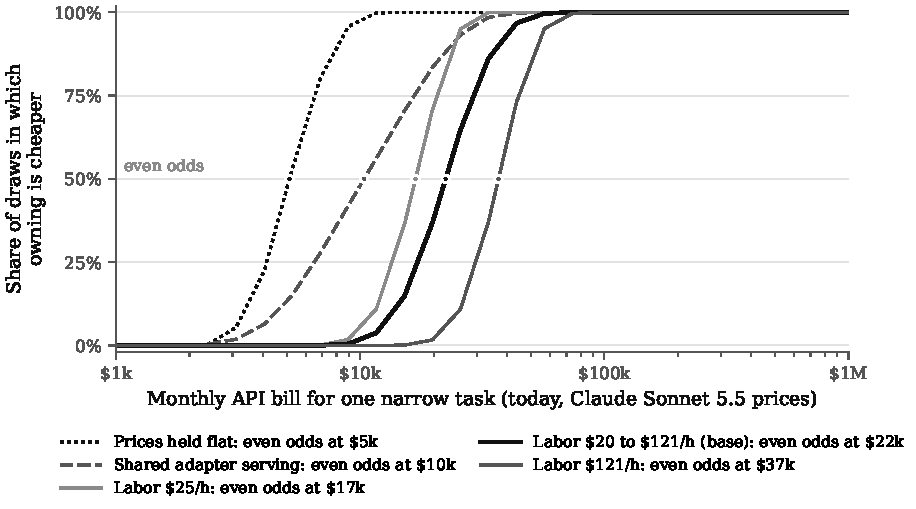
\includegraphics[width=\linewidth]{figures/fig1_ownership_curves.pdf}
\caption{Share of simulated draws in which owning a fine-tuned open 8B model is cheaper than renting Claude Sonnet 5.5 over 36 months, by today's monthly API bill for one narrow task. The shares describe the model's assumed input ranges (section~\ref{sec:math}), not the odds facing any particular organization. 20,000 draws per bill level; even-odds points interpolated on a log scale. Source: \texttt{results/econ/montecarlo\_curves.csv}.}\label{fig:curves}
\end{figure}

\lbl{Calculated} With prices and volume both held flat, owning is cheaper in half the draws at about \$5,100 a month. With falling prices and growing volume, the even-odds point is about \$22,000.

Price decline is the variable a static analysis misses. Holding prices flat while keeping growth puts the point at about \$3,000, a 7.4-fold difference. Fixing the decline at the mature-capability rate of 4.7-fold lowers it to about \$17,000.

Labor and serving move it next. At US labor rates the point is about \$37,000, and at \$25 an hour about \$17,000. Shared per-token adapter serving brings it to about \$10,000, because the idle GPU disappears.

The renter's free switching is not what drives the result. Charging the renter 10 to 40 engineering hours every time it switches models moves the point only to about \$21,700.

\begin{figure}[t]
\centering
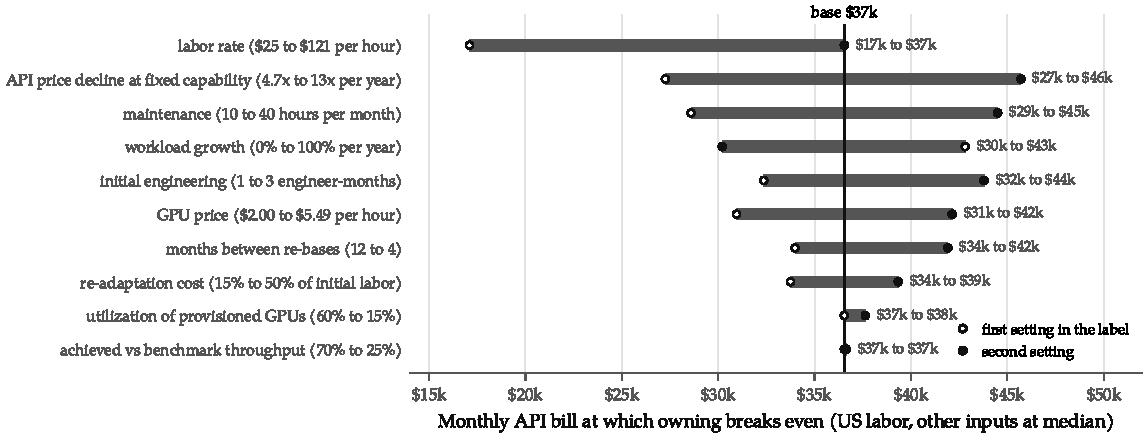
\includegraphics[width=\linewidth]{figures/fig2_sensitivity.pdf}
\caption{Sensitivity of the break-even bill to one input at a time, at US labor rates with every other input at its median (deterministic model, solved by bisection). The share of the price decline owners capture has no effect at this scale and is omitted. Source: \texttt{results/econ/tornado.csv}.}\label{fig:tornado}
\end{figure}

Figure 2 uses a deterministic version of the model. It holds every input at its median, with US labor, and moves one input at a time. Its break-even of \$36,500 sits close to the Monte Carlo even-odds point at US rates, about \$37,000. The ranking says where the decision really lies. The labor rate, the speed of API price declines and the maintenance burden move the threshold most. Utilization and serving throughput barely register, because at the break-even volume a single GPU has spare capacity. For the same reason, how much of the price decline an owner captures by re-basing has no effect at this scale, so it is not shown.

\subsection{What the model leaves out}

The model's omissions cut both ways. Three favor owning, so where they apply the true threshold is higher than reported:

\begin{itemize}
\tightlist
\item
  It ignores the 50\% batch discount, which would double the threshold for work that can wait.
\item
  It ignores negotiated enterprise discounts.
\item
  It assumes the owner matches frontier quality. Section 3 suggests that holds for behavior-shaped tasks but not knowledge-shaped ones.
\end{itemize}

Four favor renting, so where they apply the true threshold is lower:

\begin{itemize}
\tightlist
\item
  It treats each task alone, with no economies of scope across tasks that share engineers and a GPU.
\item
  It omits the value of the non-price rights in section 7.
\item
  It omits any quality \emph{gain} from owning.
\item
  It charges the renter little for migrating as models are retired.
\end{itemize}

The net direction is unknown. The point of the model is not a single number but the shape of the answer. In this model, ownership becomes likely only once a single task's API bill reaches the tens of thousands of dollars a month, and labor, not compute, sets where.

\section{The data bottleneck}\label{sec:data}

If ownership's lasting asset is the adaptation pipeline, the pipeline's weakest input is its data. Bad data matters, but mostly not for the reason usually given. A LoRA run costs a few dollars of compute, so a crashed run is cheap. The expensive failures are silent: a model that learns the wrong behavior, or an evaluation that reports the wrong accuracy and leads to the wrong decision.

\subsection{Four layers of data quality}

A training example can fail at four layers, each needing a different kind of check:

\begin{enumerate}
\def\labelenumi{\arabic{enumi}.}
\tightlist
\item
  \textbf{Syntactic.} Does the record parse and match the trainer's schema? Checked deterministically, in milliseconds.
\item
  \textbf{Structural.} Are the roles in order, the answer present, the sequence within the context window, the record unique and absent from the test set? Mostly deterministic, partly statistical.
\item
  \textbf{Semantic.} Is the answer correct? Is the preferred response actually better? This needs a model or a person.
\item
  \textbf{Representational.} Does the dataset cover the inputs the model will face in production? This needs knowledge of the deployment.
\end{enumerate}

Most tools for fine-tuning data work on the first two layers. \lbl{Hypothesis} Judging by the studies reviewed below, most of the documented harm lives in the last two.

\subsection{Five channels of harm}

Defects damage an adaptation project through different channels, and each channel has its own cost model:

{\small
\begin{longtable}[]{@{}
  >{\raggedright\arraybackslash}p{(\columnwidth - 8\tabcolsep) * \real{0.1753}}
  >{\raggedright\arraybackslash}p{(\columnwidth - 8\tabcolsep) * \real{0.2371}}
  >{\raggedright\arraybackslash}p{(\columnwidth - 8\tabcolsep) * \real{0.1753}}
  >{\raggedright\arraybackslash}p{(\columnwidth - 8\tabcolsep) * \real{0.1856}}
  >{\raggedright\arraybackslash}p{(\columnwidth - 8\tabcolsep) * \real{0.2268}}@{}}
\caption{Five channels through which data defects cost an adaptation project. \label{tab:channels}}\tabularnewline
\toprule\noalign{}
\begin{minipage}[b]{\linewidth}\raggedright
Channel
\end{minipage} & \begin{minipage}[b]{\linewidth}\raggedright
Example defects
\end{minipage} & \begin{minipage}[b]{\linewidth}\raggedright
What it costs
\end{minipage} & \begin{minipage}[b]{\linewidth}\raggedright
Evidence of harm
\end{minipage} & \begin{minipage}[b]{\linewidth}\raggedright
Caught by deterministic checks?
\end{minipage} \\
\midrule\noalign{}
\endfirsthead
\toprule\noalign{}
\begin{minipage}[b]{\linewidth}\raggedright
Channel
\end{minipage} & \begin{minipage}[b]{\linewidth}\raggedright
Example defects
\end{minipage} & \begin{minipage}[b]{\linewidth}\raggedright
What it costs
\end{minipage} & \begin{minipage}[b]{\linewidth}\raggedright
Evidence of harm
\end{minipage} & \begin{minipage}[b]{\linewidth}\raggedright
Caught by deterministic checks?
\end{minipage} \\
\midrule\noalign{}
\endhead
\bottomrule\noalign{}
\endlastfoot
Run failure & Invalid JSON, schema errors, an over-length batch that runs out of memory & Compute burned before the crash, engineer time, delay & Strong but small: crashes are loud & Yes \\
Null gradient & Exactly identical preference pairs & Wasted compute, about the defect share & Proven (5.3) & Yes \\
Gradient distortion & Concentrated duplicates, empty or truncated answers, wrong labels, near-identical pairs & Model quality & Strong for wrong labels and skewed duplication & Structural cases only \\
Measurement corruption & Train/test overlap, exact or rephrased & A biased evaluation and a wrong deployment decision & Strong and large & Exact overlap only \\
Liability & Credentials, personal data & Leakage, security and legal exposure & Strong; scales with repetition & Pattern-based, noisy \\
\end{longtable}
}

\subsection{A defect that costs nothing but compute}

Direct preference optimization (DPO) trains on pairs of a preferred answer $y_w$ and a rejected answer $y_l$ to the same prompt $x$. Its loss for one pair is

\begin{equation}\label{eq:dpo}
\mathcal{L}(\theta) = -\log \sigma\!\Big(\beta \big[\log \tfrac{\pi_\theta(y_w\mid x)}{\pi_{\text{ref}}(y_w\mid x)} - \log \tfrac{\pi_\theta(y_l\mid x)}{\pi_{\text{ref}}(y_l\mid x)}\big]\Big)
\end{equation}

If the two answers are identical, the bracket is zero for every value of the parameters $\theta$, so its gradient is zero and the loss is the constant ln 2. This holds for the standard DPO loss and for variants such as IPO that depend only on the gap between the two log-ratios. It fails once an SFT term is added, as TRL's rpo\_alpha option does, because that term still trains on the chosen answer. In a batch of $B$ pairs of which $k$ are identical, the identical pairs contribute nothing. With the usual mean over the batch, the gradient shrinks by a factor of $(B-k)/B$. That is like slightly lowering the learning rate, and an adaptive optimizer such as Adam largely rescales it away. \lbl{Observed} Section 6 confirms this in TRL with the default loss. The loss cannot tell identical pairs apart, because real pairs also start at ln 2. The gradient norm can: $2\times10^{-7}$ for identical pairs against 4.6 for real ones.

Parallelogram's documentation reports 350 identical pairs in the first 50,000 rows of UltraFeedback's preference set, 0.7\%; I did not rerun that count. Such pairs waste 0.7\% of the compute and almost nothing else. \emph{Near}-identical pairs are a different matter. Razin et al.~found that pairs with similar embeddings drive likelihood displacement: in one safety run, a Llama-3-8B model's refusal rate fell from 74.4\% to 33.4\% \citep{razin2025}. The irony is that exact-match checks catch the harmless version of this defect and miss the harmful one.

\lbl{Hypothesis} Truncation can create null-gradient pairs. Reading TRL 1.17.1's source, its DPO trainer truncates the chosen and rejected answers separately at max\_length, keeping the start. Two answers that differ only after the cutoff then become identical. I have not tested this directly.

\subsection{Finding defects one crash at a time}

When a pipeline processes data lazily, a malformed record crashes the run only when it is reached. Suppose $k$ crash-causing records sit at independent, uniformly random positions in an epoch, the run keeps no checkpoint, and a crash means starting over. The expected fraction of the epoch completed before the first crash is the expected minimum of $k$ uniform draws:

\begin{equation}\label{eq:waste}
\mathbb{E}[\text{fraction wasted}] = \frac{1}{k+1}
\end{equation}

One bad record wastes half an epoch on average before it shows itself, and ten waste 9\% before the first crash. That counts only the first crash. If each crash reveals one bad record, and the engineer fixes it and reruns, the runs end at each bad record in turn, and the expected total waste is the sum of $i/(k+1)$ for $i$ from 1 to $k$, which is $k/2$ epochs: five epochs for ten bad records. Finding defects one crash at a time is the expensive way to find them, and this is the strongest compute argument for validating data before training.

For LoRA fine-tuning it is a weak argument, for two reasons. TRL processes datasets eagerly by default, so structural crashes happen before training starts (section 6). And a LoRA epoch costs a few dollars. \lbl{Calculated} The compute value of catching crashes early is cents to dollars per run. The real costs are the engineer's debugging time and the silent harms below. The arithmetic changes for streaming pretraining or long reinforcement-learning runs, where an epoch costs thousands of dollars.

\subsection{Duplicates are hidden weights}

A duplicated example is an example with weight two. What matters is the shape of the weighting. Repeating a whole dataset for up to about four epochs is close to harmless \citep{muennighoff2023}. Concentrated repetition is not: repeating 0.1\% of the data 100 times made an 800M-parameter model perform like one half its size \citep{hernandez2022repeated}.

Duplication also drives memorization. A string seen 10 times is regenerated roughly 1,000 times more often than one seen once \citep{kandpal2022}. These three results come from pretraining, and how far they carry over to a few thousand fine-tuning rows is untested. The closest fine-tuning evidence concerns personal data: GPT-2 models fine-tuned on court cases and emails leaked personal details at measurable rates, and leakage grew roughly linearly with how often a string appeared \citep{lukas2023}. The worst combination in fine-tuning data is therefore a duplicated secret: the duplicates and secrets rules guard the same channel from two sides.

\subsection{Contamination is a decision error}

If a fraction $c$ of the test set leaked into training, the reported accuracy mixes accuracy on seen items, $a_s$, with accuracy on unseen ones, $a_u$:

\begin{equation}\label{eq:contam}
\hat{a} = (1-c)\,a_u + c\,a_s, \qquad \text{bias} = c\,(a_s - a_u)
\end{equation}

The bias can never exceed $c$. It is large only when a meaningful share of the test set leaked and the model does much better on memorized items than on new ones, that is, when the task is hard for it. Contamination is therefore most dangerous exactly when the evaluation matters most. Suppose a team ships when measured accuracy clears a threshold $\theta$. Setting sampling error aside, contamination causes a wrong decision whenever $a_u < \theta \le \hat{a}$.

The effects in the literature are large. \lbl{Observed} Training on rephrased test items lifted Llama-2-13B's MMLU score from 54.8 to 85.9, and 10-gram decontamination caught none of the rephrased items \citep{yang2023rephrased}. Some models scored up to 8\% lower on fresh grade-school math problems than on the public benchmark they resemble. That gap is consistent with contamination, but it is observational, and the authors found it only moderately correlated with signs of memorization \citep{zhang2024gsm1k}. Public fine-tuning sets carry overlap too: Yang et al.~found CodeAlpaca overlaps 12.8\% of the HumanEval test set.

\subsection{Wrong answers do harm, and systematic errors do the most}

Wrong answers in fine-tuning data do real damage. Fine-tuning Llama-3.1-8B with 30\%, 50\% and 70\% noisy responses gave MMLU scores of 59.5, 47.5 and 37.3, against 65.3 for the untuned model \citep{luo2024robustft}. That paper reports no clean fine-tuning baseline and, in the parts I read, does not say how its noise was made, so these figures measure harm against the untuned model, not against clean fine-tuning. At 100\% false responses, Llama-2-13B fell from 57.49 to 19.74 \citep{cho2024falsity}.

How much harm depends on the kind of error as well as its amount. In text classification, uniformly random label noise of 40\% cost a news task only two points with early stopping, while realistic, feature-dependent noise of about 50\% cut a Hausa task from 83.55 to 46.97 \citep{zhu2022bert}. The two numbers come from different datasets, so the contrast is suggestive rather than controlled. In long chain-of-thought data, wrong final answers cost only 3.2 points, while inserting extra steps cost 21.8 and shuffling them 10.2. Content is not irrelevant, though: corrupting every digit collapsed the score to 2.7 \citep{li2025reason}. \lbl{Hypothesis} Models average away random errors and learn consistent ones, so systematic errors, such as a labeling convention applied wrongly, are the dangerous kind. Experiment E2 in section 6 tests this in a controlled setting.

\subsection{What can be detected, and at what cost}

{\small
\begin{longtable}[]{@{}
  >{\raggedright\arraybackslash}p{(\columnwidth - 6\tabcolsep) * \real{0.2600}}
  >{\raggedright\arraybackslash}p{(\columnwidth - 6\tabcolsep) * \real{0.2200}}
  >{\raggedright\arraybackslash}p{(\columnwidth - 6\tabcolsep) * \real{0.2200}}
  >{\raggedright\arraybackslash}p{(\columnwidth - 6\tabcolsep) * \real{0.3000}}@{}}
\caption{Detectors by data-quality layer, with speed and coverage. \label{tab:detectors}}\tabularnewline
\toprule\noalign{}
\begin{minipage}[b]{\linewidth}\raggedright
Layer
\end{minipage} & \begin{minipage}[b]{\linewidth}\raggedright
Detector
\end{minipage} & \begin{minipage}[b]{\linewidth}\raggedright
Speed and cost
\end{minipage} & \begin{minipage}[b]{\linewidth}\raggedright
Catches
\end{minipage} \\
\midrule\noalign{}
\endfirsthead
\toprule\noalign{}
\begin{minipage}[b]{\linewidth}\raggedright
Layer
\end{minipage} & \begin{minipage}[b]{\linewidth}\raggedright
Detector
\end{minipage} & \begin{minipage}[b]{\linewidth}\raggedright
Speed and cost
\end{minipage} & \begin{minipage}[b]{\linewidth}\raggedright
Catches
\end{minipage} \\
\midrule\noalign{}
\endhead
\bottomrule\noalign{}
\endlastfoot
Syntactic and structural & Deterministic rules & About 8,000 rows a second on two CPU cores (section 6) & Schema, roles, empty answers, exact duplicates, exact overlap, secrets \\
Structural, fuzzy & MinHash, n-gram overlap & About 1,000 rows a second; thresholds trade recall for false flags & Near-duplicates, lightly edited overlap. True paraphrase needs embedding or model-based checks (Yang et al., 2023) \\
Semantic & A judge model, as in AlpaGasus & Dollars per 10,000 rows with a small API model & Wrong or low-quality answers, flipped preferences \\
Representational & People and production logs & Hours to weeks & Coverage gaps, distribution shift \\
\end{longtable}
}

Filtering by a judge model can pay for itself. AlpaGasus kept 9,229 of 52,002 Alpaca examples and trained 5.7 times faster. Its model won more often than it lost against the original in GPT-4 and human comparisons, and gained one to two points on standard benchmarks \citep{chen2024alpagasus}.

\textbf{Answer to the stage question.} Data validation is an enabling technology, in a narrower sense than tool marketing suggests. Deterministic checks are cheap insurance against loud failures and a handful of silent ones: empty answers, over-length rows, exact contamination, credentials in standard formats. The largest silent harms, systematic label errors and paraphrased contamination, sit beyond their reach and need statistical or model-based checks. The next section measures where those boundaries fall.

\section{An experimental investigation}\label{sec:experiments}

Three experiments test the claims of section 5. They cover what validation tools detect (E1), what a popular training framework does with bad data (E4), and how much harm each defect does (E2). All were run on a two-core CPU workspace with no GPU and no access to the Hugging Face Hub. That forced E4 and E2 onto small models built locally, which bounds what their results can show. A fourth experiment, on how fast a fine-tuned model's advantage over the frontier decays, needs GPUs and paid API calls and was not run; Appendix B gives its protocol.

\subsection{E1: what validators detect}

\textbf{Design.} I took 10,000 rows of Alpaca-cleaned (\href{https://github.com/gururise/AlpacaDataCleaned}{\texttt{gururise/AlpacaDataCleaned}}) as chat records and removed every row any tool flagged, leaving 9,963 clean rows. I did the same with 5,000 pairs from Anthropic's HH-RLHF helpful-base set (\href{https://github.com/anthropics/hh-rlhf}{\texttt{anthropics/hh-rlhf}}), leaving 4,960. Into separate copies I then injected 100 rows of each of 23 defect types at known positions. A further 1,000 Alpaca rows served as an evaluation set for the overlap checks.

Five detectors ran on every file:

\begin{itemize}
\tightlist
\item
  \textbf{Parallelogram 1.6.1}, all rules, maximum length 2,048 tokens. With no tokenizer download possible, it counted tokens approximately and reported length problems as warnings.
\item
  \textbf{The OpenAI cookbook checks}, a faithful re-implementation of its format-check loop, which tests length against a 16,385-token limit and has no secrets or personal-data checks, so its 0\% on those rows reflects its scope \citep{openai2026cookbook}.
\item
  \textbf{Exact deduplication} on each record's canonical JSON.
\item
  \textbf{MinHash near-duplicate detection}, at Jaccard similarity 0.8 on word 5-grams.
\item
  \textbf{13-gram overlap} with the evaluation set, as in the GPT-3 paper.
\end{itemize}

Ground truth is known by construction. A duplicate pair counts as caught if either member is flagged.

\textbf{Results. \lbl{Observed}} Share of injected rows flagged. Parallelogram results are marked E for error and W for warning.

{\footnotesize
\begin{longtable}[]{@{}
  >{\raggedright\arraybackslash}p{(\columnwidth - 10\tabcolsep) * \real{0.2500}}
  >{\raggedright\arraybackslash}p{(\columnwidth - 10\tabcolsep) * \real{0.2065}}
  >{\raggedright\arraybackslash}p{(\columnwidth - 10\tabcolsep) * \real{0.1630}}
  >{\raggedright\arraybackslash}p{(\columnwidth - 10\tabcolsep) * \real{0.0978}}
  >{\raggedright\arraybackslash}p{(\columnwidth - 10\tabcolsep) * \real{0.1196}}
  >{\raggedright\arraybackslash}p{(\columnwidth - 10\tabcolsep) * \real{0.1630}}@{}}
\caption{E1: share of 100 injected rows flagged, by defect type and detector. For Parallelogram, E marks an error and W a warning. \label{tab:e1}}\tabularnewline
\toprule\noalign{}
\begin{minipage}[b]{\linewidth}\raggedright
Defect
\end{minipage} & \begin{minipage}[b]{\linewidth}\raggedright
Parallelogram
\end{minipage} & \begin{minipage}[b]{\linewidth}\raggedright
OpenAI cookbook
\end{minipage} & \begin{minipage}[b]{\linewidth}\raggedright
Exact dedup
\end{minipage} & \begin{minipage}[b]{\linewidth}\raggedright
MinHash 0.8
\end{minipage} & \begin{minipage}[b]{\linewidth}\raggedright
13-gram overlap
\end{minipage} \\
\midrule\noalign{}
\endfirsthead
\toprule\noalign{}
\begin{minipage}[b]{\linewidth}\raggedright
Defect
\end{minipage} & \begin{minipage}[b]{\linewidth}\raggedright
Parallelogram
\end{minipage} & \begin{minipage}[b]{\linewidth}\raggedright
OpenAI cookbook
\end{minipage} & \begin{minipage}[b]{\linewidth}\raggedright
Exact dedup
\end{minipage} & \begin{minipage}[b]{\linewidth}\raggedright
MinHash 0.8
\end{minipage} & \begin{minipage}[b]{\linewidth}\raggedright
13-gram overlap
\end{minipage} \\
\midrule\noalign{}
\endhead
\bottomrule\noalign{}
\endlastfoot
Invalid JSON line & 100\% E & Script crashes & 0\% & 0\% & 0\% \\
Missing assistant turn & 100\% E & 100\% & 0\% & 0\% & 0\% \\
Two assistant turns in a row & 100\% E & 0\% & 0\% & 0\% & 0\% \\
Empty answer & 100\% E & 100\% & 0\% & 0\% & 0\% \\
Whitespace-only answer & 100\% E & 0\% & 0\% & 0\% & 0\% \\
Over-long answer & 98\% W & 0\% & 0\% & 0\% & 0\% \\
Over-long user context & 100\% W & 0\% & 0\% & 0\% & 0\% \\
AWS-style key in answer & 100\% E & 0\% & 0\% & 0\% & 0\% \\
GitHub token in answer & 100\% E & 0\% & 0\% & 0\% & 0\% \\
Email and phone in answer & 100\% W & 0\% & 0\% & 0\% & 0\% \\
Mojibake & 100\% W & 0\% & 0\% & 0\% & 0\% \\
Exact duplicate & 100\% E & 0\% & 100\% & 100\% & 0\% \\
Duplicate differing in whitespace & 100\% E & 0\% & 0\% & 100\% & 0\% \\
Near-duplicate (about 6\% of words edited) & 0\% & 0\% & 0\% & 16\% & 0\% \\
Exact copy of an evaluation row & 100\% E & 0\% & 0\% & 0\% & 100\% \\
Evaluation prompt, different answer & 100\% E & 0\% & 0\% & 0\% & 46\% \\
Lightly edited evaluation row (about 6\% of words) & 2\% & 0\% & 0\% & 0\% & 96\% \\
Answer swapped with another row's & 0\% & 0\% & 0\% & 0\% & 0\% \\
Answer cut off mid-sentence & 0\% & 0\% & 0\% & 0\% & 0\% \\
Identical preference pair & 100\% E & not applicable & 0\% & 0\% & not applicable \\
Empty preferred answer & 100\% E & not applicable & 0\% & 1\% & not applicable \\
Duplicate preference pair & 100\% E & not applicable & 100\% & 100\% & not applicable \\
Flipped preference pair & 0\% & not applicable & 0\% & 0\% & not applicable \\
\end{longtable}
}

No detector flagged a single untouched row in the injected files. That is true by construction, not a finding: the clean base was made by removing the 37 Alpaca rows and 40 HH pairs that any tool flagged, so it says nothing about false flags on natural data. On natural data, Parallelogram's personal-data rule warned on 57 rows of the full Alpaca set, nearly all invented example addresses and numbers, which are correct matches but not real leaks. On 5,000 HH pairs it raised 6 personal-data warnings and one encoding flag.

Three findings stand out:

\begin{enumerate}
\def\labelenumi{\arabic{enumi}.}
\tightlist
\item
  \textbf{The boundary is the semantic layer, not the tool.} Parallelogram flagged 98\% to 100\% of injected rows for 18 of the 23 defect types; the 98\% is over-long answers, counted approximately. The five types it missed are the semantic and fuzzy ones: near-duplicates, lightly edited evaluation rows, swapped answers, cut-off answers and flipped preference pairs. The other tools were not designed for most of the 23 types. None of the five detectors caught a swapped answer, a cut-off answer or a flipped preference pair. Those defects are invisible to anything that does not understand content.
\item
  \textbf{The detectors are complements.} The 13-gram check caught 96\% of lightly edited evaluation rows, where Parallelogram's exact matching caught 2\%. MinHash caught near-duplicates that exact matching missed, but only at a cost. At 0.8 it caught 16\% and flagged no untouched row. Flags on untouched rows begin at 0.7, with 2. At 0.5, recall on near-duplicates rose to about 86\% with 7 untouched rows flagged, and at 0.3 it flagged 33. Near-duplicate detection is a threshold choice, not a solved problem.
\item
  \textbf{Speed is not a constraint.} Parallelogram checked all 51,760 rows of Alpaca-cleaned in 6.4 seconds on two CPU cores, about 8,100 rows a second. MinHash ran at about 1,000 rows a second.
\end{enumerate}

\textbf{Repairs.} With \texttt{-\/-fix}, Parallelogram redacted every injected credential and personal detail, repaired the mojibake and shortened the over-long user contexts. It dropped records it could not repair, such as those with missing or empty answers or over-long answers. It left the semantic defects untouched, since it had not detected them. The repair test injected 10 rows of each of 19 single-file defect types. Of the 9,773 untouched rows, 9,767 came through unchanged. The six it dropped were the original halves of injected duplicate pairs, removed because their copy appeared earlier in the file. In three of ten whitespace-variant pairs, the padded copy survived and the clean original was removed. These counts come from a run with seed 7 that records every row's fate. The main run's seed gave 9,768 and five of ten, so the exact figures depend on where the copies land. Either way it is a minor but real flaw: deduplication should prefer the cleaner member.

\textbf{Natural defects.} The full Alpaca-cleaned set, 51,760 rows, had 4 duplicate rows and 57 rows with contact-like strings, nearly all invented examples. A random 10,000-row sample shared at least one 13-gram with a disjoint 1,000-row sample from the same set in 24 rows, so even a random split of one dataset shares some text, though some of those overlaps may be boilerplate rather than leakage. In 5,000 HH-RLHF pairs, Parallelogram found 7 identical pairs, 9 empty answers, 5 broken role sequences, 6 contact-like strings and one encoding problem.

\subsection{E4: what TRL does with bad data}

\textbf{Design.} Hugging Face's TRL is among the most widely used fine-tuning libraries. With no model downloads possible, I built a 2-layer GPT-2-style model and a byte-level BPE tokenizer locally, gave the tokenizer a ChatML template, and ran TRL 1.17.1's SFT and DPO trainers on small datasets containing one defect each. Versions: transformers 5.22.2, datasets 5.1.0, torch 2.15.0. I recorded whether each case raised an error, logged a warning, or trained silently.

\textbf{Results. \lbl{Observed}}

{\footnotesize
\begin{longtable}[]{@{}
  >{\raggedright\arraybackslash}p{(\columnwidth - 4\tabcolsep) * \real{0.2621}}
  >{\raggedright\arraybackslash}p{(\columnwidth - 4\tabcolsep) * \real{0.3204}}
  >{\raggedright\arraybackslash}p{(\columnwidth - 4\tabcolsep) * \real{0.4175}}@{}}
\caption{E4: what TRL 1.17.1 does with each defect. \label{tab:e4}}\tabularnewline
\toprule\noalign{}
\begin{minipage}[b]{\linewidth}\raggedright
Defect
\end{minipage} & \begin{minipage}[b]{\linewidth}\raggedright
TRL 1.17.1 defaults
\end{minipage} & \begin{minipage}[b]{\linewidth}\raggedright
With assistant-only loss switched on
\end{minipage} \\
\midrule\noalign{}
\endfirsthead
\toprule\noalign{}
\begin{minipage}[b]{\linewidth}\raggedright
Defect
\end{minipage} & \begin{minipage}[b]{\linewidth}\raggedright
TRL 1.17.1 defaults
\end{minipage} & \begin{minipage}[b]{\linewidth}\raggedright
With assistant-only loss switched on
\end{minipage} \\
\midrule\noalign{}
\endhead
\bottomrule\noalign{}
\endlastfoot
Invalid JSON line & Error at load, before training & Same \\
Missing assistant turn & Trains silently & Error before training \\
Unknown role names & Trains silently & Error before training \\
Empty answer & Trains silently & Trains silently \\
Conversation ends on a user turn & Not tested & Trains silently \\
Two assistant turns in a row & Not tested & Trains silently \\
Assistant speaks first & Not tested & Trains silently \\
40 copies of one example & Not tested & Trains silently \\
Rows longer than max\_length & Keeps the first 1,024 tokens and drops the rest, with a progress bar but no warning or count & Crashed in TRL's preprocessing: ``Column `assistant\_masks' doesn't exist'' \\
Identical DPO pairs & Loss ln 2, as for real pairs at the start; gradient norm $2\times10^{-7}$, against 4.6 for real pairs (learning rate $10^{-3}$, max\_length 256, not the defaults) & Not applicable \\
\end{longtable}
}

The defaults compute loss on every token and keep the start of over-long sequences. In my truncation test, each prompt alone exceeded the limit, so every answer was cut away entirely, and with default settings the model trained on prompt text alone. TRL logged no warning. With assistant-only loss switched on, missing assistant turns and unknown roles raised an error, but the message blames the tokenizer's chat template rather than the data, which sends the engineer to the wrong place.

The identical-pair result confirms section 5.3: the gradient is zero to numerical precision. One subtlety appeared: Adam still moved the parameters by 0.013 (L2 norm), against 0.49 for real pairs. Adam divides each update by a running estimate of gradient size, which amplifies floating-point noise when the true gradient is zero. The effect is small, but ``identical pairs do nothing'' is exactly true only for plain gradient descent.

\textbf{Verdict on the README's claims.} Two of Parallelogram's framework claims hold for TRL 1.17.1. Over-long samples are truncated without a warning at default settings. Duplicates are trained on silently, though I tested this only with assistant-only loss switched on. The claim that a clean exit means ``your training run won't fail because of data'' does not survive E1: semantic defects pass every check. The claims about Axolotl and Unsloth were not tested here.

\subsection{E2: how much harm each defect does}

\textbf{Design.} A small GPT-style model is pretrained on 30,000 unlabeled order sentences. It has 383,000 parameters and a word-level vocabulary. It is then fine-tuned, with loss on the answer only, on 2,000 examples of a narrow extraction task. Given a sentence such as ``can you get 7 teal kettle over to maun before friday ?'', it must return ``qty 7 item kettle color teal city maun day friday''. The test set holds 600 sentences with field combinations never seen in training.

Each defect replaces 10\% or 30\% of the fine-tuning rows and leaves everything else identical. There are five seeds, each with its own pretrained base and data. I report the change against the clean fine-tune of the same seed, with 95\% t-intervals across seeds.

The defects:

\begin{itemize}
\tightlist
\item
  \textbf{Empty answers.}
\item
  \textbf{Answers cut short} at a random word with no end token, which is what keep-start truncation does to an over-long row.
\item
  \textbf{Concentrated duplicates:} the replaced rows are copies of 20 others.
\item
  \textbf{Random label errors:} one field is wrong at random.
\item
  \textbf{Systematic label errors:} every row for a chosen set of cities carries the same wrong city. The set was chosen to cover about 10\% or 30\% of rows; the actual shares were 12.1\% and 31.9\%.
\item
  \textbf{Contamination:} test items are copied into training.
\end{itemize}

A first run at 600 fine-tuning steps was discarded. Its clean baseline reached 99.7\% on one seed and about 17\% on two, so convergence luck swamped any defect effect. The reported run uses 1,000 steps at a learning rate of $2\times10^{-3}$, where every clean fine-tune reaches 100\%. I also ran a scarce-data regime with 200 rows, in which the model does not generalize (clean accuracy 10\%). Only contamination is reported there; the other conditions in that regime sat at the floor and are kept in the bundle as uninformative.

\begin{figure}[t]
\centering
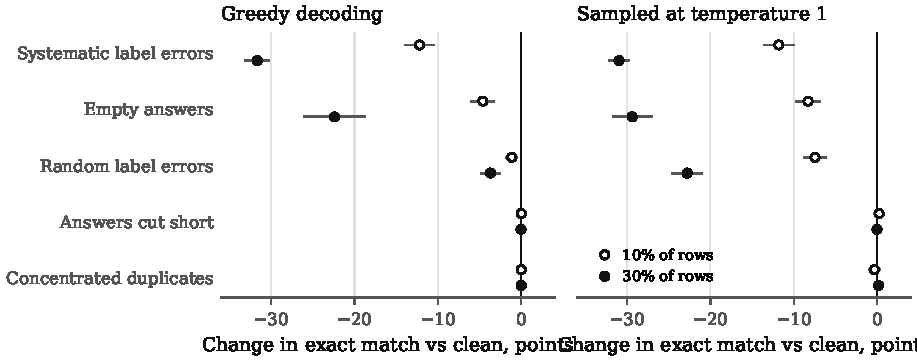
\includegraphics[width=\linewidth]{figures/fig3_e2_harm.pdf}
\caption{E2: paired change in exact-match accuracy against the clean fine-tune of the same seed; mean and 95\% t-interval over five seeds. Systematic errors affected 12.1\% and 31.9\% of rows. Source: \texttt{results/e2/e2\_summary.json}.}\label{fig:e2}
\end{figure}

\textbf{Results. \lbl{Observed}}

\begin{itemize}
\tightlist
\item
  \textbf{Systematic label errors} cost 12.2 points of accuracy when they touched 12.1\% of rows, and 31.7 points at 31.9\%. In every seed the model scored 0\% on the affected cities: it learned the mislabeling as a rule.
\item
  \textbf{Empty answers} cost 4.6 and 22.4 points. Sampled at temperature 1, the model returned nothing 7.8\% and 28.4\% of the time, close to the defect rate. It learned ``sometimes say nothing'' as a probability.
\item
  \textbf{Random label errors} cost 1.1 and 3.7 points under greedy decoding, so they were mostly averaged away. Under sampling they cost 7.5 and 22.8 points. The errors survive as probability mass that greedy decoding hides.
\item
  \textbf{Concentrated duplicates and cut-off answers} made no measurable difference at either rate.
\end{itemize}

Contamination behaved exactly as section 5.6 predicts. In the data-rich regime, leaking test items changed nothing, because the model already scored 100\% on unseen items. In the scarce-data regime it was badly misleading:

{\small
\begin{longtable}[]{@{}
  >{\raggedright\arraybackslash}p{(\columnwidth - 6\tabcolsep) * \real{0.3030}}
  >{\raggedright\arraybackslash}p{(\columnwidth - 6\tabcolsep) * \real{0.2222}}
  >{\raggedright\arraybackslash}p{(\columnwidth - 6\tabcolsep) * \real{0.2626}}
  >{\raggedright\arraybackslash}p{(\columnwidth - 6\tabcolsep) * \real{0.2121}}@{}}
\caption{E2, scarce-data regime: leaked test items inflate reported accuracy. \label{tab:contam}}\tabularnewline
\toprule\noalign{}
\begin{minipage}[b]{\linewidth}\raggedright
Test items leaked into training
\end{minipage} & \begin{minipage}[b]{\linewidth}\raggedright
Reported accuracy
\end{minipage} & \begin{minipage}[b]{\linewidth}\raggedright
Accuracy on unseen items
\end{minipage} & \begin{minipage}[b]{\linewidth}\raggedright
Inflation
\end{minipage} \\
\midrule\noalign{}
\endfirsthead
\toprule\noalign{}
\begin{minipage}[b]{\linewidth}\raggedright
Test items leaked into training
\end{minipage} & \begin{minipage}[b]{\linewidth}\raggedright
Reported accuracy
\end{minipage} & \begin{minipage}[b]{\linewidth}\raggedright
Accuracy on unseen items
\end{minipage} & \begin{minipage}[b]{\linewidth}\raggedright
Inflation
\end{minipage} \\
\midrule\noalign{}
\endhead
\bottomrule\noalign{}
\endlastfoot
None & 10.0\% & 10.0\% & none \\
10\% & 20.0\% & 11.1\% & +8.9 points \\
30\% & 35.0\% & 7.1\% & +27.9 points \\
\end{longtable}
}

With 30\% of the test set leaked, the reported accuracy was five times the true accuracy, and the leaked items scored 100\%.

\textbf{What it suggests. \lbl{Hypothesis}} The structural defects split in two. Empty answers do real harm and are cheap to catch. Duplicates at these rates and cut-off answers were close to harmless here. The most damaging defect, systematic label error, is invisible to every structural and statistical check in E1. And greedy accuracy can understate harm that appears as soon as a product samples. These are mechanisms on a small model and a synthetic task. Their size in production models is untested, and \texttt{e2\_real\_model.py} exists to test it.

\subsection{Limitations}

\begin{itemize}
\tightlist
\item
  \textbf{Scale.} E2 uses a 383,000-parameter model on a synthetic task, and E4 a tiny local model. They test mechanisms, not magnitudes in production models. The protocol in Appendix B repeats E2 on a 0.5B open model.
\item
  \textbf{Tokenizer.} Without network access, Parallelogram's length checks ran on approximate counts and reported warnings. With a model tokenizer they report errors.
\item
  \textbf{Injection realism.} Injected defects are cleaner than natural ones. Natural near-duplicates and paraphrases are more varied, so the MinHash and n-gram recall figures are optimistic. The injected credentials use the canonical AWS and GitHub key formats that pattern rules look for, so the secrets recall is optimistic too.
\item
  \textbf{Tool selection.} The defect list deliberately includes types that no structural tool, Parallelogram included, can catch, and every number above comes from scripts in Appendix B that anyone can rerun.
\end{itemize}

\section{Who should own what}

On price alone, most organizations should rent, and the ones that should own are those running one task millions of times a month at frontier prices. Price is not the only reason to own, though. For organizations whose data cannot leave the country, or whose product cannot survive a vendor's retirement schedule, ownership is a requirement, not a cost decision.

\subsection{Six cases on price}

\lbl{Calculated} These use the median assumptions of section 4 at US labor rates, over three years, discounted at 10\%. The owned option is a LoRA-tuned open 8B model at matched quality on one always-on GPU. Matched quality is generous to owning against a small rented model, but it is not the most favorable case: an owned model that beat the API on quality would do better (section 4.2).

{\footnotesize
\begin{longtable}[]{@{}
  >{\raggedright\arraybackslash}p{(\columnwidth - 12\tabcolsep) * \real{0.1875}}
  >{\raggedright\arraybackslash}p{(\columnwidth - 12\tabcolsep) * \real{0.1667}}
  >{\raggedright\arraybackslash}p{(\columnwidth - 12\tabcolsep) * \real{0.0938}}
  >{\raggedright\arraybackslash}p{(\columnwidth - 12\tabcolsep) * \real{0.1562}}
  >{\raggedright\arraybackslash}p{(\columnwidth - 12\tabcolsep) * \real{0.1562}}
  >{\raggedright\arraybackslash}p{(\columnwidth - 12\tabcolsep) * \real{0.1250}}
  >{\raggedright\arraybackslash}p{(\columnwidth - 12\tabcolsep) * \real{0.1146}}@{}}
\caption{Six cases on price: three-year discounted cost of renting and owning, at US labor rates. \label{tab:profiles}}\tabularnewline
\toprule\noalign{}
\begin{minipage}[b]{\linewidth}\raggedright
Profile
\end{minipage} & \begin{minipage}[b]{\linewidth}\raggedright
Tasks per month
\end{minipage} & \begin{minipage}[b]{\linewidth}\raggedright
Rented model
\end{minipage} & \begin{minipage}[b]{\linewidth}\raggedright
Monthly API bill
\end{minipage} & \begin{minipage}[b]{\linewidth}\raggedright
3-year cost renting
\end{minipage} & \begin{minipage}[b]{\linewidth}\raggedright
3-year cost owning
\end{minipage} & \begin{minipage}[b]{\linewidth}\raggedright
Owning $\div$ renting
\end{minipage} \\
\midrule\noalign{}
\endfirsthead
\toprule\noalign{}
\begin{minipage}[b]{\linewidth}\raggedright
Profile
\end{minipage} & \begin{minipage}[b]{\linewidth}\raggedright
Tasks per month
\end{minipage} & \begin{minipage}[b]{\linewidth}\raggedright
Rented model
\end{minipage} & \begin{minipage}[b]{\linewidth}\raggedright
Monthly API bill
\end{minipage} & \begin{minipage}[b]{\linewidth}\raggedright
3-year cost renting
\end{minipage} & \begin{minipage}[b]{\linewidth}\raggedright
3-year cost owning
\end{minipage} & \begin{minipage}[b]{\linewidth}\raggedright
Owning $\div$ renting
\end{minipage} \\
\midrule\noalign{}
\endhead
\bottomrule\noalign{}
\endlastfoot
Individual developer & 50,000 & Haiku 5.5 & \$12.50 & \$89 & \$259,915 & 2,924$\times$ \\
Individual developer needing frontier quality & 50,000 & Sonnet 5.5 & \$250 & \$1,778 & \$259,915 & 146$\times$ \\
Small company, small-model quality & 2,000,000 & Haiku 5.5 & \$500 & \$3,556 & \$259,915 & 73$\times$ \\
Small software company & 2,000,000 & Sonnet 5.5 & \$10,000 & \$71,122 & \$259,915 & 3.7$\times$ \\
Medium-sized business & 20,000,000 & Sonnet 5.5 & \$100,000 & \$711,222 & \$269,512 & 0.38$\times$ \\
Large enterprise, one task & 200,000,000 & Sonnet 5.5 & \$1,000,000 & \$7,112,220 & \$747,383 & 0.11$\times$ \\
\end{longtable}
}

The owned cost barely moves between 50,000 and 20 million tasks a month. It is almost all labor plus one always-on GPU. The individual rows are a reference point rather than a realistic plan: an individual would not pay themselves \$121 an hour or keep a data-center GPU running all month, and would use a consumer GPU or a hosted open model at about 4 cents per thousand tasks instead. Even so, the GPU floor alone, about \$2,700 a month, is eleven times their frontier API bill. For individuals, ownership is a way to learn, not a way to save.

The small software company is the interesting case. Its \$10,000 monthly bill looks large, yet owning costs nearly four times more over three years. It crosses over only if its errors are costly and an owned model is measurably better (section 4.2), or if it has a reason that is not price.

\subsection{The rights you cannot rent}

Renting gives an organization a model, but not control over that model's future. \lbl{Observed}

\begin{itemize}
\tightlist
\item
  \textbf{Retirement.} Anthropic commits to at least 60 days' notice before retiring a public model \citep{anthropic2026deprecations}. OpenAI commits to at least six months for generally available models, three for specialized variants and less for previews \citep{openai2026deprecations}. A product validated against one model snapshot must be re-validated on the vendor's schedule, not its own.
\item
  \textbf{Adaptation can be withdrawn.} OpenAI's fine-tuned models run only until their base model is retired, and OpenAI is winding down self-serve fine-tuning altogether (section 3). That is the level-2 trap in practice.
\item
  \textbf{Availability can be withdrawn.} On 12 June 2026 the US government, citing national security authorities, issued an export-control directive restricting foreign nationals' access to Claude Fable 5 and Mythos 5; secondary sources report the issuer as the Commerce Department. Unable to verify nationality in real time, Anthropic disabled both models for all customers \citep{anthropic2026fable}. The controls were lifted on 30 June. Fable 5 returned on Anthropic's own platforms on 1 July with a new classifier that routes blocked requests to Opus 4.8 and, Anthropic acknowledged, flags more benign coding requests. Mythos 5 returned only for approved US organizations \citep{anthropic2026redeploy}. Fable 5 had launched only three days before the suspension, so few products yet depended on it. The episode still shows two things a per-token price hides: access can disappear for 19 days for reasons no customer controls, and the model can come back behaving differently.
\end{itemize}

None of these risks shows up in a per-token price. Each is a reason to own at least the assets that let an organization switch quickly: its evaluation suite and its training data, which work with any model.

\subsection{Organizations with sensitive data: a view from Botswana}

Data-protection law can settle the question before economics is consulted. Botswana's Data Protection Act of 2024 prohibits transfers of personal data abroad unless the destination is designated by ministerial order. Otherwise the Information and Data Protection Commissioner must authorize the transfer, or a derogation such as the data subject's consent must apply. According to DLA Piper's summary, the designated list has about 45 entries, including South Africa, Kenya, the EU states and the UK, but not the United States \citep{dlapiper2026botswana}.

The major APIs do not offer processing in southern Africa. OpenAI's regional data processing covers the US, Europe and the UAE \citep{openai2026data}. Anthropic offers global or US-only processing, the latter at 1.1 times the standard price \citep{anthropic2026residency}. Amazon Bedrock's Cape Town region serves Claude through global cross-region inference, so computation may happen outside South Africa \citep{aws2026bedrockza}.

The two other large clouds with South African regions do not fill the gap. Microsoft's model region-availability tables list neither of its South African regions for current models; a secondary source reports a single older model on provisioned capacity, due to retire in December 2026 \citep{microsoft2026regions}. Google's Johannesburg region did not appear in the parts of its model-locations page I could load, and the same secondary source reports that it hosts custom models but not Gemini \citep{google2026locations}.

\lbl{Hypothesis} For a Botswana hospital, bank or ministry processing personal data, the simplest compliant route to a capable model may be open weights served in Botswana or in a South African cloud region. For them, the break-even analysis of section 4 is beside the point. The comparison is with the cost of authorizations, consent flows and the uses forgone without them. This is an analysis of incentives, not legal advice, and the Act's commencement date and designations should be checked against the Government Gazette.

\lbl{Speculation} The same logic applies wherever residency law is strict and in-country API processing is absent. It may be the strongest single driver of model ownership outside the largest economies.

\subsection{Decision rules}

\begin{enumerate}
\def\labelenumi{\arabic{enumi}.}
\tightlist
\item
  \textbf{If the task depends on knowledge that changes, use retrieval, not fine-tuning.} In controlled tests, retrieval beat unsupervised fine-tuning for injecting new knowledge (section 3).
\item
  \textbf{If a prompted small API model meets the quality bar, rent it.} At \$0.25 per thousand tasks it costs less than any owned setup at these volumes. Only a hosted open model, at about \$0.04 per thousand, is cheaper, and that is renting too.
\item
  \textbf{If a narrow task needs frontier quality and its API bill runs to tens of thousands of dollars a month, test a fine-tuned open model.} In my model the even-odds point is about \$22,000 a month at a median labor rate of about \$50 an hour, and about \$37,000 at US rates. Own at level 3 where shared adapter serving is available, and at level 4 otherwise.
\item
  \textbf{If errors are expensive, measure the quality gap before the price gap.} A few points of accuracy can outweigh the entire token bill.
\item
  \textbf{If data cannot leave, ownership is a requirement.} Budget for it as compliance, not as a saving.
\item
  \textbf{Whatever you decide, own the data and the evaluations.} They are the only assets that survive a change of model, rented or owned.
\end{enumerate}

\section{The coming decade}

The future of model ownership turns on four variables: how fast rented capability gets cheaper, how much labor adaptation needs, whether adapters can be served cheaply on shared infrastructure, and how often governments and vendors restrict access to rented models. None of these is fixed, and the most important of them is moving fastest. Everything in this section is conditional, and labeled as projection or speculation.

\subsection{What the trends say, read cautiously}

\lbl{Calculated} If the share of AI builders who post-train kept growing at its 2025 to 2026 rate, 1.67-fold a year, it would reach about 17\% in 2027 and 28\% in 2028. That rests on one year-on-year change in one survey, so treat it as an upper-end illustration, not a forecast. The open-weight share of enterprise tokens rebounded from 11\% to 19\% in the same year, after falling the year before, while its share of spend fell from 6\% to 4\% \citep{menlo2026}. Tokens measure use, not ownership: an open-weight token may well be served by a third-party host. If both trends continue, open models will carry a growing share of the work and a shrinking share of the money, which is what a commodity looks like.

\subsection{Four scenarios}

\textbf{A. The rented frontier.} The closed frontier pulls ahead on agentic work, API prices keep falling at 13-fold a year or faster, and vendors add in-region processing where residency law demands it. Ownership stays where it is today: a minority of AI-native companies, plus residency niches. \emph{Conditions:} the open-weight lag widens beyond six months, and in-region processing arrives in markets such as southern Africa.

\textbf{B. The bifurcated stack.} Organizations rent the frontier for open-ended reasoning and run adapted open models for high-volume narrow tasks, mostly through partners. What they own is data, evaluations and adapters, not hardware. Post-training keeps growing; open models' share of tokens rises while their share of spend stays small. \emph{Conditions:} roughly today's trends continue. \lbl{Speculation} I consider this the most likely of the four over the next five years.

\textbf{C. The adapter economy.} Shared adapter serving becomes standard and cheap again, adapters move between providers, and base-model families change less often, so adapters live longer. In my model, pooled serving cuts the bill at which owning becomes likely from about \$22,000 to about \$10,000 a month (section 4). That would bring mid-sized companies into ownership. \emph{Conditions:} per-token adapter serving returns at base-model prices, after its 2026 retreat at Together.

\textbf{D. The sovereignty shock.} Export controls, sanctions, data-localization laws or prolonged outages make dependence on foreign APIs a board-level risk. Ownership becomes insurance and is priced as such. \emph{Conditions:} more episodes like the June 2026 export-control suspension of Fable 5 and Mythos 5, or residency laws spreading faster than in-region API processing.

The scenarios are not exclusive. B with a dose of D is plausible, especially outside North America and Europe.

\subsection{The variable that may move most}

Section 4 found that labor, not compute, sets the ownership threshold: the even-odds point is about \$37,000 a month at US labor rates and about \$17,000 at \$25 an hour. \lbl{Speculation} Labor is also the input that AI itself is reducing fastest. Coding agents already write and maintain much of the data tooling, training scripts and evaluation harnesses an adaptation pipeline needs. \lbl{Calculated} In my model, cutting the engineering, review and maintenance hours tenfold lowers the even-odds point from about \$22,400 to about \$12,800 a month. Cheaper labor alone stops there, because one always-on GPU remains. Combine it with shared adapter serving and the point falls to about \$1,100 a month, about twenty-one times lower. At that level ownership reaches organizations that cannot consider it today. \lbl{Speculation} The strongest force for model ownership in the coming decade may be the models themselves, doing the work of owning, together with infrastructure that lets many owners share a GPU.

This cuts both ways. The same agents make it easier to migrate between rented models, which lowers the cost of renting too.

\subsection{Signposts}

{\small
\begin{longtable}[]{@{}
  >{\raggedright\arraybackslash}p{(\columnwidth - 6\tabcolsep) * \real{0.2828}}
  >{\raggedright\arraybackslash}p{(\columnwidth - 6\tabcolsep) * \real{0.3131}}
  >{\raggedright\arraybackslash}p{(\columnwidth - 6\tabcolsep) * \real{0.1818}}
  >{\raggedright\arraybackslash}p{(\columnwidth - 6\tabcolsep) * \real{0.2222}}@{}}
\caption{Signposts for the coming decade, with their latest readings. \label{tab:signposts}}\tabularnewline
\toprule\noalign{}
\begin{minipage}[b]{\linewidth}\raggedright
Signpost
\end{minipage} & \begin{minipage}[b]{\linewidth}\raggedright
Latest reading
\end{minipage} & \begin{minipage}[b]{\linewidth}\raggedright
Source
\end{minipage} & \begin{minipage}[b]{\linewidth}\raggedright
Ownership more likely if it\ldots{}
\end{minipage} \\
\midrule\noalign{}
\endfirsthead
\toprule\noalign{}
\begin{minipage}[b]{\linewidth}\raggedright
Signpost
\end{minipage} & \begin{minipage}[b]{\linewidth}\raggedright
Latest reading
\end{minipage} & \begin{minipage}[b]{\linewidth}\raggedright
Source
\end{minipage} & \begin{minipage}[b]{\linewidth}\raggedright
Ownership more likely if it\ldots{}
\end{minipage} \\
\midrule\noalign{}
\endhead
\bottomrule\noalign{}
\endlastfoot
Open-weight lag behind the frontier & About 4 months (May 2026) & \citealp{edwards2026gap} & Narrows, especially on agentic tasks \\
Price decline at fixed capability & About 13-fold a year since 2023 & \citealp{emberson2026price} & Slows \\
Open-weight share of enterprise tokens and spend & 19\% of tokens, 4\% of spend & \citealp{menlo2026} & Spend share starts rising \\
AI builders who post-train & 10\%, up from 6\% & \citealp{menlo2026} & Keeps rising, with more done in-house \\
H100 rental index & Headline about \$3.00 an hour (\$2.53 in the same page's FAQ), about 27\% above May 2025 & \citealp{silicondata2026h100} & Falls \\
Shared adapter serving & Discontinued at Together in 2026 & \citealp{together2026lora} & Returns at base-model prices \\
Closed-vendor fine-tuning & OpenAI winding down, 2026--27 & \citealp{openai2026deprecations} & More vendors exit \\
In-country API processing in southern Africa & None among major APIs & Section 7.3 & Stays absent \\
Access suspensions of rented models & One, in 2026: 19 days; Fable 5 returned with changed behavior, Mythos 5 only for approved US organizations & \citealp{anthropic2026fable} & Recur \\
\end{longtable}
}

\section{Synthesis}\label{sec:synthesis}

\textbf{Will organizations increasingly own and adapt their AI capabilities rather than exclusively rent them?} Yes, in the narrow sense the question asks, and the best evidence is post-training rather than token share. The share of AI builders who post-train rose from 6\% to 10\% in a year, in one survey. Open models' share of enterprise tokens rebounded from 11\% to 19\%, but tokens measure use, not ownership. And the framing of renting versus owning hides what the evidence here shows. Almost no one is moving from rented frontier models to owned ones. Organizations are adding an owned layer underneath a rented one.

\subsection{What the evidence supports}

\begin{itemize}
\tightlist
\item
  \textbf{Rented intelligence keeps the money.} \lbl{Observed} Closed models take about 96\% of enterprise spend while carrying about 81\% of tokens. Capability, not price, decides purchases, and the frontier remains rented.
\item
  \textbf{Ownership on price alone is rare.} \lbl{Calculated} For one narrow task, owning a fine-tuned model comes out cheaper in half the simulated draws only once the monthly API bill reaches about \$22,000, and about \$37,000 at US labor rates. That even-odds point holds for the model's assumed input ranges, not for any particular organization. Holding API prices flat in the same model puts it about seven times lower, which is why a static analysis overstates the case for owning.
\item
  \textbf{A cost advantage is perishable.} \lbl{Calculated} At observed price declines, a tenfold cost advantage lasts one to two years. Lifetime savings are capped at 4.7 to 7.8 months of today's API bill for that workload with flat volume, and 5.4 to 10 months with median growth. Both figures assume a renter who moves to cheaper models for free.
\item
  \textbf{Labor sets the threshold, not compute.} \lbl{Calculated} At the break-even point one GPU has spare capacity, and two thirds of the cost of owning is people.
\item
  \textbf{The strongest reasons to own are not about price.} \lbl{Hypothesis} They are availability, retirement schedules, residency law, and errors that cost more than tokens. Residency bites hardest where in-country API processing does not exist, as in southern Africa, the only region I checked.
\item
  \textbf{Data defects matter mainly through silent harm.} \lbl{Observed} In E1, Parallelogram flagged 98\% to 100\% of injected rows for 18 of 23 defect types, all structural or pattern-based, at about 8,000 rows a second. None of the five detectors caught swapped answers, cut-off answers or flipped preferences. At default settings, TRL trained silently on most of the structural defects tested. In E2, systematic label errors cost up to 32 points of accuracy and are invisible to structural checks. Empty answers cost up to 22 points and are cheap to catch. Random errors that greedy decoding hides cost up to 23 points once the model samples. Rephrased contamination, the largest harm in the literature, also lies beyond structural checks.
\end{itemize}

\subsection{What remains uncertain}

Five things limit these conclusions. The harm experiments ran on small models, so real-model magnitudes are untested; the script to test them is ready. The decay of the specialization premium, the mechanism at the center of section 4, is argued but not measured. Adoption of fine-tuning in production is not measured by anyone. The price trends that drive the model are three years old, averaged across benchmarks, and may not persist; GPU prices have already reversed once. And the residency argument rests on one region; I did not survey others.

\subsection{What this means for developers}

Treat the model as the most replaceable part of the system, because on current trends it will be replaced, by the vendor or by you, within a year or two. Spend on the parts that survive the replacement:

\begin{itemize}
\tightlist
\item
  a dataset that defines the task precisely
\item
  an evaluation suite that is provably separate from it
\item
  a pipeline that can re-adapt the next base model in days rather than months
\end{itemize}

Measure quality in the currency of errors, not tokens. And validate data in layers: cheap structural checks on every commit, statistical checks for near-duplicates and overlap, and model-based checks where errors are expensive.

\subsection{Where validation fits}

Validation does not earn its keep by saving GPU hours; for LoRA runs it barely does, and in my model re-adaptation cost moves the ownership threshold only modestly. Its value is narrower and more durable. The dataset and the evaluation suite are the assets that outlive every model, and validation keeps them trustworthy as they are reused. Structural checks are the cheapest layer of that protection, and E1 and E2 show where that layer stops.

\subsection{A closing observation}

The price of a fixed level of machine intelligence is falling faster than that of any technology Epoch has measured, including computing, batteries and DNA sequencing, though Epoch itself cautions that comparisons across such different technologies are loose. When something gets cheaper that fast, owning the thing itself is rarely the advantage. The advantage goes to whoever can say precisely what they want from it, and check that they got it.

The usual question is whether to rent or own a model. A better question is what an organization would have to rebuild if its model disappeared tomorrow. For most, the honest answer is not weights and not GPUs. It is the examples that define the job and the tests that show whether the job is done. Those are worth owning outright, whoever's model happens to be running this year.

\appendix

\section{Notation and model details}

{\small
\begin{longtable}[]{@{}
  >{\raggedright\arraybackslash}p{(\columnwidth - 4\tabcolsep) * \real{0.1373}}
  >{\raggedright\arraybackslash}p{(\columnwidth - 4\tabcolsep) * \real{0.4412}}
  >{\raggedright\arraybackslash}p{(\columnwidth - 4\tabcolsep) * \real{0.4216}}@{}}
\caption{Notation and the values or ranges used in the model. \label{tab:notation}}\tabularnewline
\toprule\noalign{}
\begin{minipage}[b]{\linewidth}\raggedright
Symbol
\end{minipage} & \begin{minipage}[b]{\linewidth}\raggedright
Meaning
\end{minipage} & \begin{minipage}[b]{\linewidth}\raggedright
Value or range used
\end{minipage} \\
\midrule\noalign{}
\endfirsthead
\toprule\noalign{}
\begin{minipage}[b]{\linewidth}\raggedright
Symbol
\end{minipage} & \begin{minipage}[b]{\linewidth}\raggedright
Meaning
\end{minipage} & \begin{minipage}[b]{\linewidth}\raggedright
Value or range used
\end{minipage} \\
\midrule\noalign{}
\endhead
\bottomrule\noalign{}
\endlastfoot
$c, c_R, c_O$ & Inference cost per task: in general, renting, owning & From list prices; section 2 \\
$s, s_R, s_O$ & Task success rate & Assumed equal in the simulation \\
$c_{\mathrm{err}}$ & Cost of catching and fixing one failed task & Worked example only \\
$F$ & One-off adaptation cost: engineering, data review, labeling, compute & Engineering 160 to 480 hours; review 40 to 120 hours; 2,000 to 10,000 labeled examples \\
$T$ & Useful life of an adapted model & Set by re-base interval \\
$M$ & Monthly upkeep: maintenance hours plus the idle cost of the always-on GPU & 10 to 40 hours, plus one GPU at h per hour while volume is below its capacity \\
$V$ & Tasks per month & Derived from the API bill \\
$A_0$ & Today's monthly API bill for the workload & Swept from \$100 to \$3 million \\
$\lambda_A$ & Continuous rate at which rented cost per task falls & ln 4.7 to ln 13 per year \\
$\lambda_O$ & Rate at which owned cost falls in the simulation, through re-basing & $\varphi\lambda_A$ at each re-base, $\varphi$ from 0.3 to 1 \\
$\lambda_{\mathrm{chip}}$ & Rate at which owned cost falls with hardware alone, for an owner who never re-bases; used in the half-life table & ln 1.49 per year \\
$g$ & Workload growth rate & 0 to ln 2 per year \\
$h$ & GPU price per hour & \$2.00 to \$5.49 \\
$u$ & Utilization of provisioned GPUs & 15\% to 60\% \\
$\kappa$ & Cost of an input token relative to an output token & 0.1 to 0.4 \\
$\delta$ & Discount rate & 10\% per year \\
\end{longtable}
}

\textbf{Task.} 1,500 input and 200 output tokens. The rented comparator is Claude Sonnet 5.5 at \$2 and \$10 per million input and output tokens.

\textbf{Capacity.} Start from 14,992 output tokens per second for Llama 3.1 8B on one H100 at 1,000 input and 1,000 output tokens \citep{nvidia2026trtllm}. Convert input tokens to output-equivalents at weight $\kappa$, then scale by an efficiency factor of 25\% to 70\% for real-world serving.

\textbf{Serving.} Cost is the larger of one always-on GPU (730 hours a month) and the GPU-hours the volume needs at utilization $u$. In the level-3 scenario, serving is instead billed per token at one to three times DeepInfra's Llama 3.1 8B price, with no idle floor.

\textbf{Re-basing.} Every $T_b$ months, from 4 to 12, the owner re-adapts onto a newer base at 15\% to 50\% of the initial engineering hours. Owned unit costs then step down by $\exp(-\lambda_O T_b)$.

\textbf{Rent.} The monthly bill follows $A_0 \exp\big((g-\lambda_A)\,t\big)$, which assumes the renter migrates to cheaper models of equal capability as they appear.

\textbf{Comparison.} Both sides are discounted over 36 months. Owning ``wins'' a draw when its discounted cost is lower.

\textbf{Monte Carlo.} 20,000 draws per bill level across 40 log-spaced bill levels. Labor is sampled log-uniformly from \$20 to \$121 an hour, a median of about \$49, or fixed at \$121 or \$25 in the labor scenarios. The even-odds point is the bill at which owning wins half the draws, interpolated on a log scale between grid levels. Bisection at median parameters is used only for the sensitivity chart, which moves one input at a time to the ends of its range.

\section{Reproducibility and open questions}

Every original number in this essay comes from a script in the accompanying repository, \href{https://github.com/Thatayotlhe04/a-parallel-paradigm}{\texttt{github.com/Thatayotlhe04/a-parallel-paradigm}}, which also holds the raw outputs and the typeset LaTeX version of this essay.

\subsection{Environment}

Two-core x86-64 CPU, 7 GB RAM, no GPU, no access to the Hugging Face Hub. Python 3.13, torch 2.15.0, transformers 5.22.2, datasets 5.1.0, trl 1.17.1, peft 0.21.2, parallelogram 1.6.1, datasketch 1.18.1, numpy 2.5.4, pandas 3.1.1, scipy 1.18.1.

\subsection{Data}

{\small
\begin{longtable}[]{@{}
  >{\raggedright\arraybackslash}p{(\columnwidth - 4\tabcolsep) * \real{0.3455}}
  >{\raggedright\arraybackslash}p{(\columnwidth - 4\tabcolsep) * \real{0.3455}}
  >{\raggedright\arraybackslash}p{(\columnwidth - 4\tabcolsep) * \real{0.3091}}@{}}
\caption{Data files and their SHA-256 hashes. \label{tab:data}}\tabularnewline
\toprule\noalign{}
\begin{minipage}[b]{\linewidth}\raggedright
File
\end{minipage} & \begin{minipage}[b]{\linewidth}\raggedright
Source
\end{minipage} & \begin{minipage}[b]{\linewidth}\raggedright
SHA-256
\end{minipage} \\
\midrule\noalign{}
\endfirsthead
\toprule\noalign{}
\begin{minipage}[b]{\linewidth}\raggedright
File
\end{minipage} & \begin{minipage}[b]{\linewidth}\raggedright
Source
\end{minipage} & \begin{minipage}[b]{\linewidth}\raggedright
SHA-256
\end{minipage} \\
\midrule\noalign{}
\endhead
\bottomrule\noalign{}
\endlastfoot
alpaca\_data\_cleaned.json & \href{https://github.com/gururise/AlpacaDataCleaned}{\texttt{gururise/AlpacaDataCleaned}}, main branch & {\ttfamily\footnotesize\seqsplit{bd844b8247a0f543804b6ce0882b0aaec4bbf5e8d66167df6213a0f1e4fe878b}} \\
helpful-base/train.jsonl.gz & \href{https://github.com/anthropics/hh-rlhf}{\texttt{anthropics/hh-rlhf}}, master branch & {\ttfamily\footnotesize\seqsplit{518a5bf288456fc9f3b7c980c54116fba0c52f274d3f4d344675d83e4058f6f4}} \\
\end{longtable}
}

\subsection{Scripts, seeds and outputs}

{\small
\begin{longtable}[]{@{}
  >{\raggedright\arraybackslash}p{(\columnwidth - 6\tabcolsep) * \real{0.3305}}
  >{\raggedright\arraybackslash}p{(\columnwidth - 6\tabcolsep) * \real{0.2034}}
  >{\raggedright\arraybackslash}p{(\columnwidth - 6\tabcolsep) * \real{0.1017}}
  >{\raggedright\arraybackslash}p{(\columnwidth - 6\tabcolsep) * \real{0.3644}}@{}}
\caption{Scripts, seeds and outputs. \label{tab:scripts}}\tabularnewline
\toprule\noalign{}
\begin{minipage}[b]{\linewidth}\raggedright
Script
\end{minipage} & \begin{minipage}[b]{\linewidth}\raggedright
What it does
\end{minipage} & \begin{minipage}[b]{\linewidth}\raggedright
Seeds
\end{minipage} & \begin{minipage}[b]{\linewidth}\raggedright
Output
\end{minipage} \\
\midrule\noalign{}
\endfirsthead
\toprule\noalign{}
\begin{minipage}[b]{\linewidth}\raggedright
Script
\end{minipage} & \begin{minipage}[b]{\linewidth}\raggedright
What it does
\end{minipage} & \begin{minipage}[b]{\linewidth}\raggedright
Seeds
\end{minipage} & \begin{minipage}[b]{\linewidth}\raggedright
Output
\end{minipage} \\
\midrule\noalign{}
\endhead
\bottomrule\noalign{}
\endlastfoot
\texttt{e1\_detection.py} & E1 defect injection and detection & 20261108 & \texttt{results/e1/e1\_results.json} \\
\texttt{e1b\_followup.py} & E1 MinHash threshold trade-off & as E1 & \texttt{results/e1/e1b\_results.json} \\
\texttt{e1c\_fix\_fate.py} & E1 repair outcomes from Parallelogram's per-line log & 7 & \texttt{results/e1/e1c\_results.json} \\
\texttt{e4\_trl\_audit.py} & E4 TRL behavior with a local tiny model & 0, 1 & \texttt{results/e4/e4\_results.json} \\
\texttt{e4b\_defaults\_truncation.py} & E4 default settings and truncation & 1 & \texttt{results/e4/e4b\_results.json} \\
\texttt{e2\_harm.py} & E2 harm dose-response, 5 seeds & 0 to 4 & \texttt{results/e2/e2\_runs.jsonl} (80 runs); the discarded 600-step pilot and the uninformative 200-row runs are kept as \texttt{e2\_runs\_pilot\_600steps.jsonl} and \texttt{e2\_runs\_dropped\_lowdata.jsonl} \\
\texttt{e2\_analyze.py} & E2 paired differences against the clean run of each seed, with t-intervals & none & \texttt{results/e2/e2\_summary.csv} and \texttt{.json} \\
\texttt{econ\_model.py} & Section 4 model, Monte Carlo and sensitivity, plus named scenarios: static prices, labor rates, pooled serving, mature-capability decline, renter switching costs, labor hours cut tenfold, and the section 4.2 worked example & 20261108 & \texttt{results/econ/} \\
\texttt{make\_figures.py} & Figures 1 to 3 from the result files & none & \texttt{paper/figures/} \\
\texttt{e2\_real\_model.py} & E2 on a real 0.5B model; not run here & 0 to 2 & (for GPU users) \\
\end{longtable}
}

To reproduce: create a Python 3.13 environment with the versions above, download the two data files, check their hashes, and run each script with the arguments in its docstring. Run them with \texttt{python\ -I} so nothing in the data directories can shadow a library. One figure is not reproduced by these scripts: the 350 identical UltraFeedback pairs in section 5.3 come from Parallelogram's public-datasets documentation.

\subsection{Protocol for E3, not run here}

E3 tests the central mechanism of section 4: whether a fine-tuned model's lead over a prompted frontier model shrinks as base models improve.

\begin{enumerate}
\def\labelenumi{\arabic{enumi}.}
\tightlist
\item
  Take one narrow behavioral task with exact-match scoring, such as structured extraction.
\item
  Fine-tune the same 5,000-example dataset, with the same LoRA settings, on at least three generations of one open small-model family released 6 to 12 months apart.
\item
  Score each against the same 1,000-item held-out set, alongside the untuned base and a prompted frontier API model.
\item
  Report the fine-tuning lift over each base, and the gap to the frontier model, with confidence intervals over three seeds.
\item
  A shrinking lift across generations measures the specialization-premium decay that feeds T in section 4. A stable lift argues for longer model lifetimes and lower ownership thresholds.
\end{enumerate}

Estimated cost: nine runs of 5,000 examples, one epoch each. For an 8B model family that is about 21 hours on a T4-class GPU, scaled from Labonne's T4 timing; a 1B to 3B family needs a fraction of that. API calls for the frontier comparison cost under \$20.

\subsection{Open questions}

\begin{itemize}
\tightlist
\item
  How many organizations hold adapters in production? No public dataset measures it.
\item
  How do my injected-defect recall figures compare with natural defects in proprietary datasets?
\item
  Does TRL's separate truncation of chosen and rejected answers create identical DPO pairs in practice, and how often?
\item
  What do Axolotl and Unsloth do with each defect type?
\item
  Do E2's small-model effects hold at 0.5B to 8B parameters? \texttt{e2\_real\_model.py} is ready for anyone with a GPU.
\end{itemize}
